\section{Theory}

\subsection{The Cost Function }
\label{sec:cost_fn}

\label{sec:theory}

** the model in (ADL, 1993),
we consider a cost function of the form

\begin{equation}
  \label{eq:cost-t_d}
  C(t_d; \alpha, \beta, \gamma, t^*) = \alpha tt(t_d) + \beta[t^*-t_d-tt(t_d)]^+ + \gamma[t_d+tt(t_d)-t^*]^+ 
\end{equation}
where
\begin{itemize}
\item \(t_d\) is a possible departure time, on which the cost depends
\item \(t^*\) is the desired arrival time
\item \(\alpha\) is the value of time spent travelling
\item \(\beta\) is the value of time spent waiting there
\item \(\gamma\) is the value of time arriving late
\item \(tt(t_d)\) is the time spent travelling if leaving at time \(t_d\)
\item \([x]^+ = \max(0, x)\)
\end{itemize}

We will consider, in this article,
how the cost depends on the time at which a person arrives,
rather than the time at which the person departs.
Since the travel time is known without uncertainty,
the users will then be able to make a choice based on their arrival time.

Let thus
\begin{equation}
  \label{eq:t_a-t_d}
  t_a(t_d) = t_d + tt(t_d)
\end{equation}
be the function linking the departure time to the arrival time.
The following holds:
\begin{obs}
  \label{obs:inv-t_a}
  The function \(t_a(t_d)\) is invertible
\end{obs}
This simply follows from noting that  \(t_a(t_d)\) must be strictly increasing:
this corresponds to the traffic following a First In First Out (FIFO) logic,
that is, a later departure cannot result in an earlier arrival:
a reasonable assumption that we make on the travel time function.

The function \(t_d(t_a)\) that, given an arrival time,
yields the unique departure time that would result in the given arrival,
is thus well defined.
The travel time function can hence be defined in term of the arrival time:
\begin{definition}
  \label{def:tta}
  Let
  \begin{equation*}
    tt:\R \rightarrow \R
  \end{equation*}
  be a function expressing the travel time in terms of the departure time.
  The function \(tt_a\), expressing the travel time in terms of the arrival time, is defined as follows:
  \begin{equation*}
    tt_a(t_a) = tt(t_d(t_a))
  \end{equation*}
\end{definition}

The assumption of the traffic following a FIFO logic has different implications,
on the functions \(tt\) and \(tt_a\):

\begin{lemma}
  \label{lemma:bounded-der-tt}
  Suppose the travel time functions \(tt, tt_a\) to be differentiable.
  
  The traffic follows a First In First Out logic if and only if the function \(tt\) satisfies
  \begin{equation*}
    tt'(t_d) > -1\quad \forall \, t_d
  \end{equation*}
  or, equivalently, the function on arrival time \(tt_a\) satisfies
  \begin{equation*}
    tt_a'(t_a) < 1\quad \forall \, t_a
  \end{equation*}
\end{lemma}
\begin{proof}
  Note that the traffic follows a FIFO logic if and only if the function \(t_a(t_d)\) is strictly increasing,
  and, once defined, its inverse \(t_d(t_a)\) will be so.
  
  Being \(t_a(t_d)\) differentiable, it is increasing if and only if its derivative is positive:
  \begin{align*}
    \diffp{}{{t_d}} t_a(t_d) & > 0 \\
    1 + tt'(t_d) & > 0 \\
    tt'(t_d) & > -1
  \end{align*}
  
  Alternatively, consider its inverse
  \begin{equation*}
    t_d(t_a) = t_a - tt_a(t_a)
  \end{equation*}

  Again, it is increasing if and only if it has positive derivative:
  \begin{align*}
    \diffp{}{{t_a}} t_d(t_a) & > 0 \\
    1 - tt_a'(t_a) & > 0 \\
    tt_a'(t_a) < 1
  \end{align*}
\end{proof}

Once this needed property on the travel time function was stated,
the cost function can be simplified by expressing it in function of the arrival time:
by using equation \eqref{eq:t_a-t_d} and Definition~\ref{def:tta},
the expression for the cost in~\eqref{eq:cost-t_d} indeed simplifies,
becoming

\begin{equation}
  \label{eq:cost-t_a}
  C(t_a; \alpha, \beta, \gamma, t^*) = \alpha tt_a(t_a) + \beta[t^*- t_a]^+ + \gamma[t_a - t^*]^+ 
\end{equation}
where the dependency of \(t_a\) on the departure time \(t_d\) has been hidden:
the arrival time can indeed be directly observed,
and its dependency on the departure time neglected.

In the following article,
the expression used will be the one given the arrival time, as shown in~\eqref{eq:cost-t_a},
being that a simpler expression if compared to the original one in~\eqref{eq:cost-t_d}.

We will, lastly normalize \(\alpha\) to 1.
This is possible since the cost can be considered up to a multiplicative constant.
Instead of the real cost \(C\) we will thus consider a scaled version of it \(C/\alpha\),
and minimize the following:
\begin{equation}
  \label{eq:cost_final}
  C(t_a; \beta, \gamma, t^*) = tt_a(t_a) + \beta[t^*- t_a]^+ + \gamma[t_a - t^*]^+ 
\end{equation}

The notation is here ambiguous regarding the cost \(C\) and the coefficients \(\beta,\gamma\).
It anyway doesn't lose in generality, and was chosen for simplicity.

\subsection{Minimum of the Cost Function}
\label{sec:cost_minima}

Consider hence the cost in \eqref{eq:cost_final},
and the problem of finding the minimum of it.
Before computing the first order condition,
in order to find the global minimum it is useful to do some qualitative reasoning on the values taken by the cost function.

Note that, indeed, a value \(t_0\) for the arrival time can only be greater,
smaller or equal to the given \(t^*\).
In the following definition,
the two cases are separated, so that they can be studied independently.
\begin{definition}
  Let values for the parameters \(\beta, \gamma, t^*\) be fixed.
  \begin{itemize}
  \item The \textbf{optimal early arrival} \(t_e^{opt}\) is the early arrival realizing the least cost:
    \begin{equation*}
      t_e^{opt}(\beta, \gamma ,t^*) = \argmin_{t_a < t^*}C(t_a; \beta, \gamma, t^*)
    \end{equation*}
  \item The \textbf{optimal late arrival} \(t_l^{opt}\) is the late arrival realizing the least cost:
    \begin{equation*}
      t_l^{opt}(\beta, \gamma ,t^*) = \argmin_{t_a > t^*}C(t_a; \beta, \gamma, t^*)
    \end{equation*}
  \item The \textbf{optimal arrival} \(t^{opt}\) is the arrival realizing the least cost:
    \begin{equation*}
      t^{opt}(\beta, \gamma ,t^*) = \argmin_{t_a}C(t_a; \beta, \gamma, t^*)
    \end{equation*}
  \end{itemize}
\end{definition}

Please note that in general,
optimal early and late arrivals may not exist,
depending on the choice of the travel time function and the parameters.
The zones in which these minima exist will be studied later.

For studying where these minima occur, consider now the case of an early arrival \(t_a = t_0 < t^*\).
Since
\begin{equation*}
  t_0 - t^* < 0
\end{equation*}
the cost simplifies, becoming
\begin{align}
  C(t_0; \beta, \gamma, t^*) & = tt_a(t_0) + \beta[t^*- t_0]^+ + \gamma[t_0 - t^*]^+ \nonumber \\
                             & = tt_a(t_0) + \beta(t^*- t_0)\label{eq:cost_early}
\end{align}

\begin{figure}
  \centering
  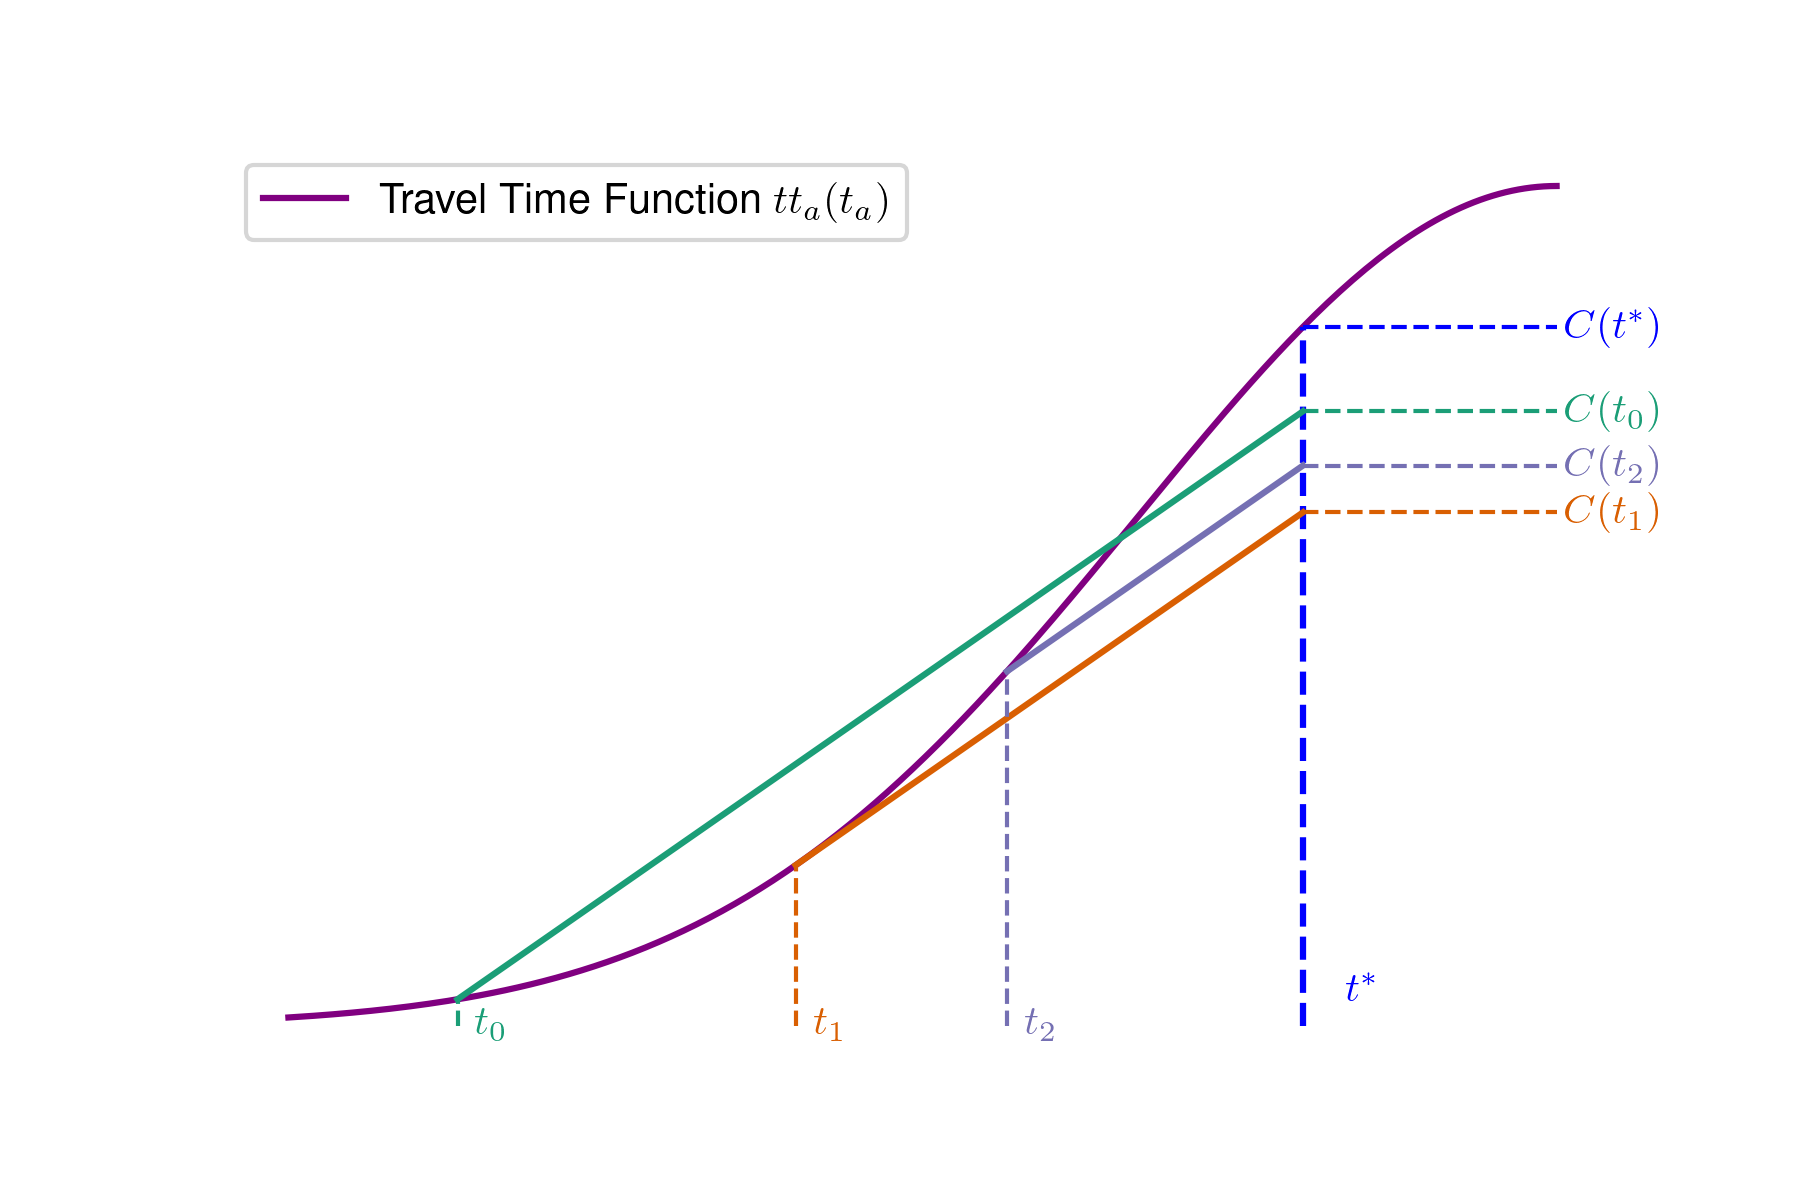
\includegraphics[width=.8\textwidth]{early_arrivals_cost}
  \caption{Dependency of the cost on the arrival time, for early arrival.
    The solid lines are parallel, of slope \(\beta\).
  Note that their distance is the only factor affecting the cost of an early arrival}
  \label{fig:early_arrivals_cost}
\end{figure}

The cost will thus be, as expected,
the sum of the travel time and a term linear on the distance of the actual arrival from the desired one.

Figure \ref{fig:early_arrivals_cost} displays how the cost of an early arrival changes when varying the arrival time:
the cost is only determined by the distance of the lines of slope \(\beta\) between each other, that is,
the projected distance of the points \(tt_a(t_a)\) on the axis orthogonal to the lines determining the cost
(the one described by \(y = -x/\beta\)).

This reasoning leads to the following lemma:
\begin{lemma}
  \label{lemma:cost_decoupled}
  If an optimal early arrival \(t_e^{opt}\) exists,
  it can be found by solving a simple minimization problem:
  \begin{equation*}
    t_e^{opt} = \argmin_{t_a < t^*} (tt_a(t_a) - \beta t_a)
  \end{equation*}

  Similarly, if an optimal late arrival exists,
  it is
  \begin{equation*}
    t_l^{opt} = \argmin_{t_a > t^*} (tt_a(t_a) + \gamma t_a)
  \end{equation*}
\end{lemma}
\begin{proof}
  The claim for early arrivals simply follows from the expression for the cost in~\eqref{eq:cost_early}:
  the following indeed holds for \(t_a < t^*\)
  \begin{align*}
    C(t_a; \beta, \gamma, t^*) & = tt_a(t_a) + \beta(t^*- t_a) \\
                               & = tt_a(t_a) + \beta t^* - \beta t_a
  \end{align*}

  But \(\beta t^*\) is clearly constant in \(t_a\),
  and minimization is invariant on translations.
  This yields
  \begin{align*}
    t_e^{opt} & = \argmin_{t_a < t^*} C(t_a) \\
              & = \argmin_{t_a < t^*} (tt_a(t_a) + \beta t^* - \beta t_a) \\
              & = \argmin_{t_a < t^*} (tt_a(t_a) - \beta t_a)
  \end{align*}

  Regarding late arrivals, the argument is symmetrical and thus omitted.
\end{proof}

Note that this has some trivial implication on the value of the derivative of the travel time function at the optimal points:
\begin{obs}
  \label{obs:foc}
  The derivative of the travel time function \(tt_a'\) is fixed at the optimal points:
  \begin{itemize}
  \item \(tt_a'(t_e^{opt}) = \beta\)
  \item \(tt_a'(t_l^{opt}) = -\gamma\)
  \end{itemize}
\end{obs}

This follows from the Lemma above:
if the function \(tt_a\) is differentiable, being the minima computed over an open set,
if they exist they necessarily satisfy the first order conditions.
For the early arrivals, they are
\begin{align*}
  \diffp{}{{t_a}} \left(tt_a(t_a) - \beta t_a\right) & = 0 \\
  tt_a'(t_a) & = \beta
\end{align*}
The case for late arrival is analogous.

While not particularly difficult to retrieve,
the expression in Lemma~\ref{lemma:cost_decoupled} is useful,
since it makes a clearer decoupling of the dependencies of the point that minimizes the cost on the parameters \(\beta, \gamma\) and \(t^*\).
We can indeed see how changing the parameters affects the location of the points \(t_e^{opt}, t_l^{opt}\).
This is described by the following proposition:
\begin{prop}
  Given a value for the parameters \(\beta, \gamma\),
  there exists a collection of disjoint intervals
  \begin{equation*}
    E = \{(t_e^i, \bar{t_e^i})\}_i,\quad i = 1, \dots, n
  \end{equation*}
  such that, if exists a value for \(i\) such that \(t^* \in (t_e^i, \bar{t_e^i})\),
  the optimal early arrival will be the lower bound of the interval:
  \begin{equation*}
    t_e^{opt}(\beta, \gamma, t^*) = t_e^{i}
  \end{equation*}

  If such a value for \(i\) does not exist,
  then the optimal early arrival is not defined.
\end{prop}

\begin{proof}
  Proof
\end{proof}

\begin{figure}
  \centering
  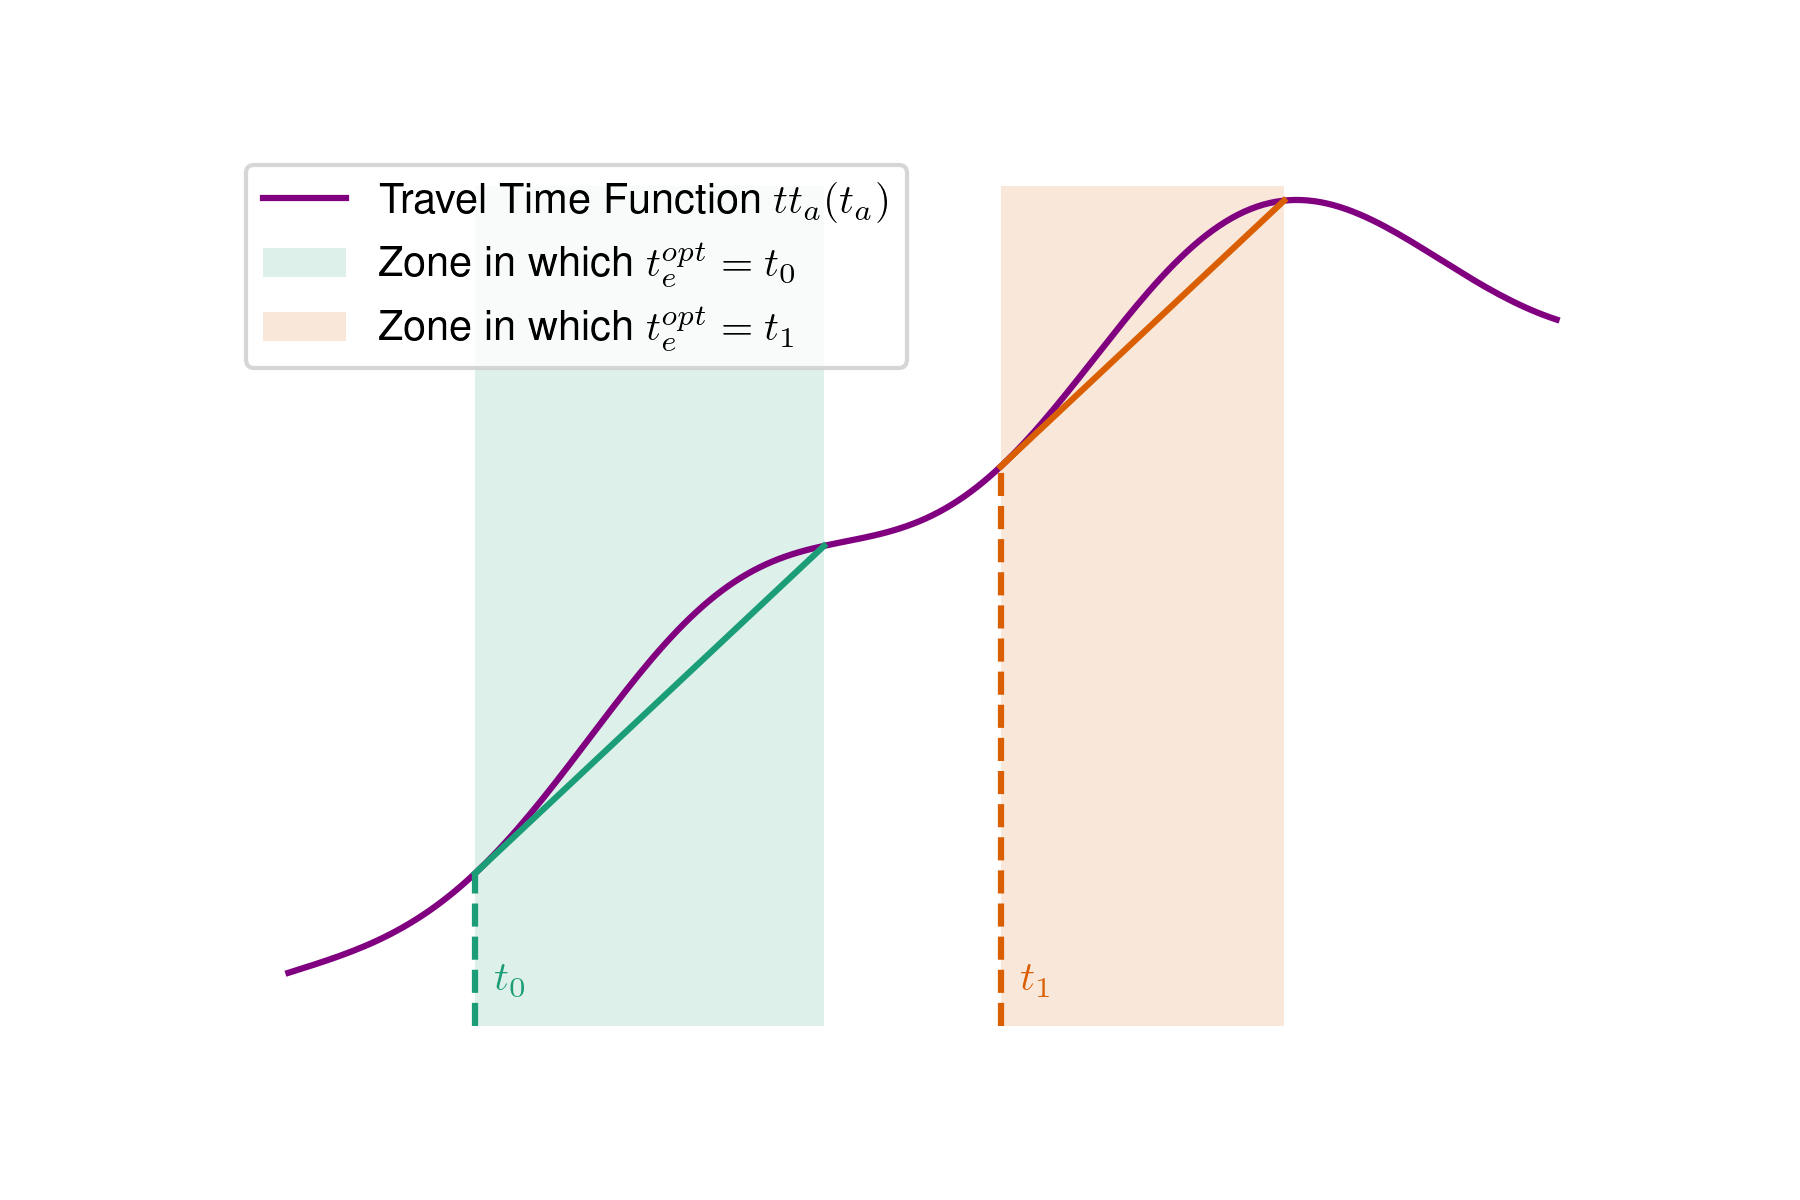
\includegraphics[width=.8\textwidth]{early_arrivals_jump}
  \caption{How the optimal early arrival changes,
    when changing the parameter \(t^*\).
    When \(t^*\) is in one of the shaded zones,
    the optimal early arrival time \(t_e^{opt}\) will be constant and equal to the time that yielded the zone.
  Otherwise, the optimal early arrival does not exist.}
  \label{fig:early_arrivals_jump}
\end{figure}

Figure~\ref{fig:early_arrivals_jump} shows this behaviour:
when \(t^*\) falls in the shaded zones,
the optimal early arrival \(t_e^{opt}\) is constant (in each of the zones).
If \(t^*\) is not in the zones,
the optimal early arrival is not defined:
for these values of the parameter,
the global minimum will be realized by either an on-time arrival (that is, \(t^{opt} = t^*\))
or by a late arrival.

The case of late arrival is, as expected, exactly symmetrical.

Once the dependency of the points \(t_e^{opt}, t_l^{opt}\) on the parameters has been explained,
the global minimum \(t^{opt}\) has to be characterized.
To this end, note that the optimum can only be smaller, greater or equal to \(t^*\):
\begin{obs}
  \label{obs:t_opt-dep}
  Given values for the parameters \(\beta, \gamma, t^*\) one out of the following is always true:
  \begin{itemize}
  \item \(t^{opt} = t_e^{opt}\) that is, the optimal arrival is an early arrival
  \item \(t^{opt} = t_l^{opt}\) that is, the optimal arrival is a late arrival
  \item \(t^{opt} = t^*\) that is, the optimal arrival is an on-time arrival
  \end{itemize}
\end{obs}

While the characterization of the points \(t_e^{opt}, t_l^{opt}\) is straightforward and done above,
describing the interaction between early and late arrivals is in general not easy,
and can be made simpler by assuming the travel time function to have some realistic features.

\begin{definition}
  \label{def:gen-tt-fun}
  Consider a function
  \begin{equation*}
    tt_a: \R \rightarrow \R
  \end{equation*}

  \(tt_a\) is said a \textbf{general travel time function} if it satisfies the following:
  \begin{enumerate}
  \item \(tt_a \in C^1(\R)\)\todo{Add limits to \(\pm\infty\). Adapt later, where it says \textit{first requirement} etc}
  \item \(tt_a'(t_a) < 1\ \forall\, t_a\in \R\)
  \item \(tt_a\) is unimodal
  \end{enumerate}
\end{definition}

The first requirement is not restrictive,
since the space \(C^1(\R)\) is dense in the space of continuous functions,
and the travel time function can be assumed to be continuous.
Requirement about the bounded derivative arises from Lemma~\ref{lemma:bounded-der-tt}.
Unimodality, finally, is a restrictive requirement that has never been mentioned earlier,
and simplifies the problem of describing the interactions of early and late arrivals.
It is anyway realistic:
if considering only one out of the morning and evening peak (that can be treated separately),
we indeed expect the traffic pattern to be unimodal\todo{Cite something}.

Under these assumptions, when a set of parameters results in an early or late arrival can be clearly stated:
it is indeed possible to find a point before which the arrivals can only be either early or on-time,
and after which the arrivals can only be late or on-time:

\begin{prop}
  Let \(tt_a\) be a general travel time function, the parameters \(\beta, \gamma\) be given.
  There exists a point \(t_s(\beta, \gamma) \in \bar{\R} = \{\R \cup \pm \infty\}\) that satisfies
  \begin{itemize}
  \item \(t^{opt}(\beta, \gamma, t^*) \neq t_e^{opt}(\beta, \gamma, t^*)\) if \(t^* > t_s(\beta, \gamma)\)
  \item \(t^{opt}(\beta, \gamma, t^*) \neq t_l^{opt}(\beta, \gamma, t^*)\) if \(t^* < t_s(\beta, \gamma)\)
  \end{itemize}

  Moreover, when \(t^* = t_s(\beta, \gamma)\) arriving early or late yields the same cost:
  \begin{equation*}
    C(t_e^{opt}(\beta, \gamma, t_s); \beta, \gamma, t_s) = C(t_l^{opt}(\beta, \gamma, t_s); \beta, \gamma, t_s)
  \end{equation*}
\end{prop}
\begin{proof}
  
  
  % To prove the first part of the proposition,
  % it is enough to show that if 
  If there is no point realizing a late arrival, that is
  \begin{equation*}
    \nexists\, t^* |\, t^{opt}(t^*) = t_l^{opt}(t^*)\footnote{For the scope of this proposition, how the parameters \(\beta, \gamma\) change is not relevant:
  for notational simplicity, the dependency of the points \(t^{opt}, t_e^{opt}, t_l^{opt}\) on these parameters are thus hidden,
  and the only dependency to be explicitly denoted will be the one on the desired arrival time \(t^*\).}
  \end{equation*}
  then the proposition is true, for \(t_s = \infty\).

  Otherwise, consider a point \(t_0\) realizing a late arrival:
  \begin{equation*}
    t^{opt}(t_0) = t_l^{opt}(t_0)
  \end{equation*}

  We will now prove that a desired arrival time later than \(t_0\) cannot yield an early arrival:
  in the following, is shown that, given \(t_1 > t_0\),
  \begin{equation*}
    t^{opt}(t_1) \neq t_e^{opt}(t_0)
  \end{equation*}

  The proof will be divided in two different cases:
  \(t_1\) can be either greater or smaller than \(t_l^{opt}(t_0)\).

  At first, we suppose it to be smaller: \[t_1 \leq t_l^{opt}(t_0)\]

  This case will be again divided in two different cases:
  \(t_e^{opt}(t_1)\) can be either greater than \(t_0\) or smaller.

  Suppose now the second case:
  \begin{equation*}
    t_e^{opt}(t_1) \leq t_0
  \end{equation*}
  In this case, arrival at \(t_l^{opt}(t_0)\) is a realizable late arrival when the desired arrival time is \(t_1\) as well.
  Its cost will be lower than the cost of the same arrival,
  when the desired arrival time is \(t_0\):
  this is because the cost decreases on the distance between the desired arrival time (in this case, \(t_1\)) and the actual arrival time (in this case, \(t_l^{opt}(t_0)\)).
  \begin{align*}
    C(t_l^{opt}(t_0); \beta, \gamma, t_1) & = tt_a(t_l^{opt}(t_0)) + \gamma(t_l^{opt}(t_0) - t_1) \\
                                          & < tt_a(t_l^{opt}(t_0)) + \gamma(t_l^{opt}(t_0) - t_0) \\
                                          & = C(t_l^{opt}(t_0); \beta, \gamma, t_0)
  \end{align*}
  Moreover, the cost of every possible early arrival increases:
  the arrival time \(t_e^{opt}(t_1)\) is, on top of this, a realizable early arrival even when the desired arrival time is \(t_0\),
  and its cost is lower in this case:
  similarly, to the earlier computations,
  \begin{align*}
    C(t_e^{opt}(t_1); \beta, \gamma, t_1) & = tt_a(t_e^{opt}(t_1)) + \beta(t_1 - t_e^{opt}(t_1)) \\
                                          & > tt_a(t_e^{opt}(t_1)) + \beta(t_0 - t_e^{opt}(t_1)) \\
                                          & = C(t_e^{opt}(t_1); \beta, \gamma, t_0)
  \end{align*}
  There exists thus, when the desired arrival time is \(t_0\),
  a late arrival whose cost is lower than the one of the best early arrival:
  \begin{align*}
    C(t_l^{opt}(t_0); \beta, \gamma, t_1) & < C(t_l^{opt}(t_0); \beta, \gamma, t_0) \\
                                          & < C(t_e^{opt}(t_1); \beta, \gamma, t_0) \\
                                          & < C(t_e^{opt}(t_1); \beta, \gamma, t_1)
  \end{align*}

  Consider now the case in which the optimal early arrival is greater than the desired arrival \(t_0\):
  \begin{equation*}
    t_e^{opt}(t_1) > t_0
  \end{equation*}

  In this case, the travel time function has to be increasing at \(t_e^{opt}(t_1)\),
  being it an early arrival (as shown in Observation~\ref{obs:foc}),
  and by unimodality it has to be increasing at \(t_0\) as well.
  The cost of a late arrival at \(t_l^{opt}(t_0)\) is, on the other hand, decreasing:
  \begin{equation}
    \label{eq:cost-comp-1}
    \begin{split}
      C(t_l^{opt}(t_0); \beta, \gamma, t_1) & = tt_a(t_l^{opt}(t_0)) + \gamma(t_l^{opt}(t_0) - t_1) \\
                                            & < tt_a(t_l^{opt}(t_0)) + \gamma(t_l^{opt}(t_0) - t_0) \\
                                            & = C(t_l^{opt}(t_0); \beta, \gamma, t_0)
    \end{split}
  \end{equation}

  Moreover, the optimality of \(t_l^{opt}(t_0)\), when the desired arrival time is \(t_0\), yields
  \begin{equation}
    \label{eq:cost-comp-2}
    \begin{split}
      C(t_l^{opt}(t_0); \beta, \gamma, t_0) & < C(t_0; \beta, \gamma, t_0) \\
                                            & = tt_a(t_0)
    \end{split}
  \end{equation}

  Suppose now \(t_e^{opt}(t_1) > t_0\).

  Being the function \(tt_a\) increasing, its value in \(t_e^{opt}(t_1)\) will be greater than at \(t_0\):
  \begin{equation}
    \label{eq:decreasing-tt_a}
    tt_a(t_0) \leq tt_a(t_e^{opt}(t_1))
  \end{equation}

  Finally, the cost of an arrival at \(t_e^{opt}(t_1)\) will be lower bounded by the travel time:
  \begin{equation}
    \label{eq:cost-low-bound}
    \begin{split}
      C(t_e^{opt}(t_1); \beta, \gamma, t_1) & = tt_a(t_e^{opt}(t_1)) + \beta(t_1 - t_e^{opt}(t_1)) \\
                                            & > tt_a(t_e^{opt}(t_1))
    \end{split}
  \end{equation}

  By using equations \eqref{eq:cost-comp-1}, \eqref{eq:cost-comp-2}, \eqref{eq:decreasing-tt_a} and \eqref{eq:cost-low-bound},
  we get
  \begin{align*}
    C(t_e^{opt}(t_1); \beta, \gamma, t_1) & > tt_a(t_e^{opt}(t_1)) \\
                                          & \geq tt_a(t_0) \\
                                          & > C(t_l^{opt}; \beta, \gamma, t_0) \\
                                          & > C(t_l^{opt}(t_0); \beta, \gamma, t_1)
  \end{align*}
  showing that there is a late arrival whose cost is smaller than the best early arrival for \(t_1\).


  Consider, finally, the case in which \[t_1 > t_l^{opt}(t_0)\]

  Note that the reasoning above shows, given the arbitrariness of the choice of \(t_1\),
  \begin{align*}
    C(t_e^{opt}(t_1); \beta, \gamma, t_1) & > C(t_l^{opt}(t_0); \beta, \gamma, t_l^{opt}(t_0)) \\
                                          & = tt_a(t_l^{opt}(t_0))
  \end{align*}
  where, in the last line, the cost has been computed.

  Note now that the function \(tt_a\) has to be decreasing (again, given Observation~\ref{obs:foc}) at \(t_l^{opt}(t_0)\) and,
  as a consequence of unimodality,
  will be so until \(t_1\). This implies
  \begin{equation*}
    tt_a(t_1) \leq tt_a(t_l^{opt}(t_0))
  \end{equation*}

  The value of the travel time is a lower bound for the optimal cost,
  being it the cost of an on-time arrival.
  An early arrival will thus not be realized,
  since the cost for an on-time arrival will be lower:
  \begin{align*}
    C(t_1; \beta, \gamma, t_1) & = tt_a(t_1) \\
                               & \leq tt_a(t_l^{opt}(t_0)) \\
                               & = C(t_l^{opt}(t_0); \beta, \gamma, t_l^{opt}(t_0)) \\
                               & < C(t_e^{opt}(t_1); \beta, \gamma, t_1)
  \end{align*}

  This shows that \(t_1\) cannot yield an early arrival,
  if the function \(tt_a\) is decreasing at \(t_0\).

  This reasoning shows that, given a desired arrival time that realizes a late arrival,
  a greater desired arrival time will never yield an early arrival.

  A symmetric reasoning will show the same for early arrivals:
  given a desired arrival time that yields an early arrival,
  no earlier desired arrival times will yield late arrivals.

  These two statements prove the first part of the proposition:
  let indeed
  \begin{align*}
    t_{s, l} & = \inf\{t^* |\, t^{opt}(t^*) = t_l^{opt}(t^*)\} \\
    t_{s, e} & = \sup\{t^* |\, t^{opt}(t^*) = t_e^{opt}(t^*)\}
  \end{align*}

  Any choice of \(t_s \in [t_{s, e}, t_{s, l}]\) will satisfy the two requirements for \(t_s\).

  Regarding the second part of the proposition,
  that is, that the cost of arriving early or late at \(t_s\) is the same,
  it simply follows from a careful choice of the value \(t_s\).

  Note indeed that the cost of arriving early continuously grows as the value of \(t_s\) is increased from \(t_{s, e}\),
  while the cost of arriving late continuously grows as \(t_s\) is decreased from \(t_{s, l}\).

  Since the cost of arriving late when desiring \(t_{s, e}\) is greater than the cost of arriving early,
  and the cost of arriving early when desiring \(t_{s, l}\) is greater than the cost of arriving late,
  there has to be a value for \(t_s\) that satisfies the claim.\todo{Better argue this}
\end{proof}


%%% Local Variables:
%%% mode: LaTeX
%%% TeX-master: "../main"
%%% End:
